\documentclass[10pt]{article}
\usepackage[a4paper,margin=1.6cm]{geometry}
\usepackage{graphicx,booktabs,amsmath,microtype,multicol,xcolor,hyperref,enumitem,caption}
\hypersetup{colorlinks=true,urlcolor=blue!60!black,linkcolor=black}
\setlist{nosep,leftmargin=1.2em}
\setlength{\parskip}{3pt}\setlength{\parindent}{0pt}
\captionsetup{font=small,skip=3pt}
\setlength{\columnsep}{0.7cm}
\usepackage[compact]{titlesec}
\titlespacing*{\section}{0pt}{6pt}{2pt}
\titleformat*{\section}{\large\bfseries}
\renewcommand{\arraystretch}{1.05}

\begin{document}
\begin{center}
{\Large\bfseries Predicting Summer Olympic Medal Counts: Replicating and Extending\\``2020 Summer Olympics Predictions Using Machine Learning''}\\[4pt]
UE24CS352A Machine Learning, Mini-Project \#53\\
\textit{Team: [Name 1 (SRN)], [Name 2 (SRN)]} \quad$\cdot$\quad Code: \texttt{[GitHub repository URL]}
\end{center}
\vspace{-4pt}
\raggedcolumns
\begin{multicols}{2}

\section*{1\quad Problem statement}
Given a country's economic and demographic indicators, its team size and its medal count at the previous Games,
predict how many medals it wins at a Summer Olympics. We replicate the CS229 report by Dobkowski (2021)
and extend it. The paper could only test on Rio 2016, because Tokyo 2020 had not yet taken place. We also predict
Tokyo 2020 and score against the real medal table.

\section*{2\quad Dataset}
\begin{itemize}
\item \textbf{Kaggle ``120 years of Olympic history''}: 271k athlete-event rows, 1896--2016. Team events are
  counted once (deduplicated on Games + event + medal + NOC), which gives the official medal-table totals
  (e.g.\ USA 2016 = 121).
\item \textbf{World Bank WDI} (REST API): GDP, GDP per capita, GDP growth, population, population growth, land area,
  plus world totals for the \% of world GDP and population.
\item \textbf{Tokyo 2020} medal table (1,080 medals, 93 NOCs) and team sizes (205 NOCs), scraped from Wikipedia.
\end{itemize}
One row is one country at one Games, from 1988 onward (the paper avoids the 1980/84 boycotts): 1,734 rows.
NOC codes are mapped to ISO3 codes, folding historical teams into successor states
(URS/EUN$\to$RUS, FRG/GDR$\to$DEU, ROC$\to$RUS). Some codes collide with another ISO3 country
(NOC BRN is Bahrain; ISO BRN is Brunei). Rows missing any indicator are dropped (e.g.\ USSR 1988, North Korea,
Chinese Taipei), which leaves \textbf{1,650 rows}. 60\% of them have zero medals.
The 13 features follow the paper's Table 1: year, GDP, GDP/capita, GDP growth, \% world GDP, population,
\% world population, population growth, land area, medals last Games, total medals awarded, athletes, \% athletes.

\section*{3\quad Approach}
\textbf{Two-stage model.} The target has a large point mass at zero, so a \emph{classifier} first predicts whether
a country wins any medal. A \emph{regressor} trained only on medal winners then predicts the count, and countries
classified as non-winners get 0. Classifiers: logistic regression, SVM, Gaussian NB, MLP, random forest.
Regressors: linear, locally weighted linear ($w_i=e^{-(y_i-y_0)^2/2\tau^2}$), ridge, lasso, Poisson, SVR
(linear/poly/RBF/sigmoid kernels), random forest. All features are standardised.

\textbf{Objective.} Eq.\,1 is the MSE over all countries. Eq.\,2 is the MSE over the ten countries with the
most actual medals. Regressors are selected on Eq.\,1\,+\,0.25\,Eq.\,2. We report RMSE, the paper's ``average
standard deviation''.

\textbf{Protocol.} Hyperparameters are tuned with 5-fold Grid/Randomized search on 1988--2008.
\emph{Paper protocol}: select on 2012, refit on 1988--2012, test on 2016.
\emph{Our protocol}: a single validation year is noisy, so every classifier$\times$regressor pair (and single-stage
regression) is scored with rolling-origin validation (train on all Games before $Y$, predict $Y$, for
$Y\in\{2004,2008,2012\}$). Both selected models are then refit on 1988--2016 to predict \textbf{Tokyo 2020}.

\section*{4\quad Implementation}
Python with pandas and scikit-learn. The modules are: WDI download, Tokyo scraper, NOC$\to$ISO3 mapping, dataset
builder, model zoo with search spaces and a \texttt{TwoStageModel} estimator, metrics, training script, feature
ablation, paper audit, and figures. A Streamlit app is used for the demo. It covers predictions for any model pair and
year, model comparison tables, a country explorer, and a what-if tool on the Tokyo 2020 model.
\texttt{run\_all.sh} rebuilds everything from the raw CSVs in about a minute.

\section*{5\quad Results}
\textbf{Stage 1 (2012).} Tuned accuracies: logistic regression 0.888, SVM 0.883, random forest 0.883,
MLP 0.868, Gaussian NB 0.868. These are close to the paper's 0.855--0.891; always predicting ``no medal'' scores 0.57.
\textbf{Stage 2 (2012, behind logistic regression).} Tuning fixed SVR (10.50$\to$2.88) and improved ridge
(3.13$\to$2.85). Random forest had the lowest error with default parameters (2.52).

\begin{center}
\small
\begin{tabular}{@{}lcc@{}}
\toprule
RMSE (medals / country) & Rio 2016 & Tokyo 2020\\
\midrule
Naive: same as last Games & \textbf{3.28} & 3.68\\
Linear regression (baseline) & 3.31 & 3.43\\
Paper protocol: LogReg + Ridge & 3.66 & 3.40\\
Rolling protocol: Random Forest & 3.57 & \textbf{3.07}\\
\midrule
\textit{Paper's reported GNB + Ridge} & \textit{2.26} & --\\
\bottomrule
\end{tabular}
\end{center}

\begin{center}
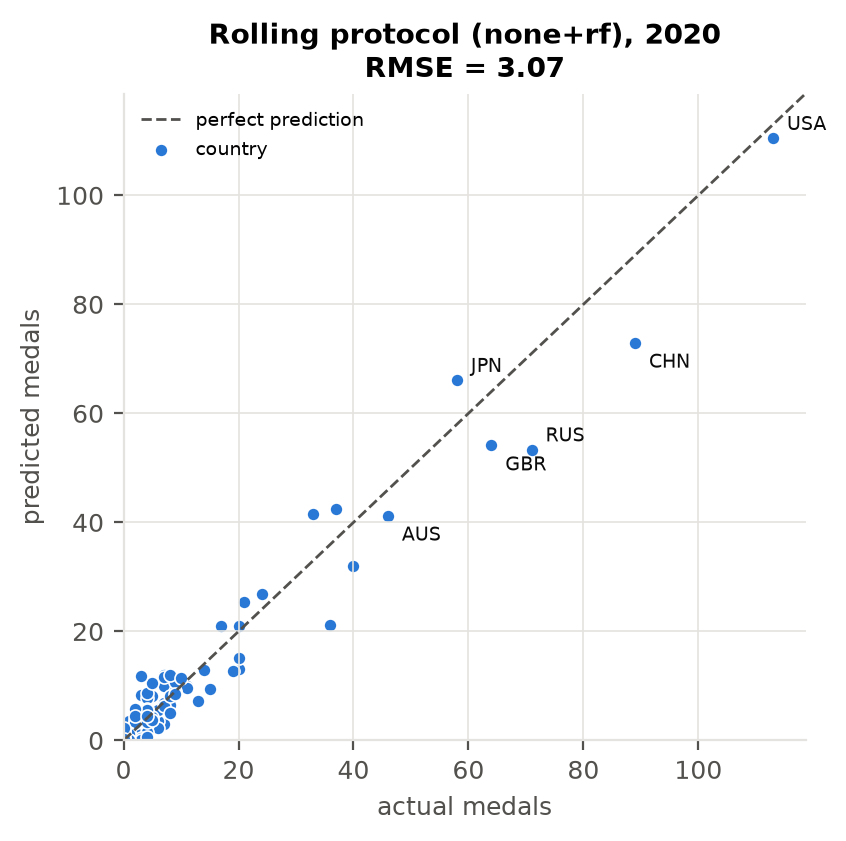
\includegraphics[width=0.82\columnwidth]{../figures/fig6_final_2020.png}
\captionof{figure}{Tokyo 2020: predicted vs actual medals for the rolling-protocol model (random forest).}
\end{center}

On Tokyo 2020 the rolling-protocol random forest beats the linear baseline by 0.36 and the naive guess by 0.61
(USA 110 vs 113, host Japan 66 vs 58). The largest misses are China (73 vs 89), ROC (53 vs 71) and the Netherlands
(21 vs 36). These are countries whose results move a lot from one Games to the next.

\textbf{Checking the paper's 2016 result.} We could not reproduce RMSE 2.26: the same model gives 3.66 on
held-out 2016 data. The ``actual 2016'' counts in the paper's Table 4 are the \emph{2012} counts:

\begin{center}
\footnotesize\setlength{\tabcolsep}{3.5pt}
\begin{tabular}{@{}lccccc@{}}
\toprule
 & USA & CHN & GBR & DEU & JPN\\
\midrule
Paper ``actual 2016'' & 103 & 89 & 65 & 44 & 38\\
True 2012 & 103 & 88 & 65 & 44 & 38\\
True 2016 & 121 & 70 & 67 & 42 & 41\\
Paper predicted & 103 & 85 & 52 & 44 & 45\\
Ours, in-sample 2012 & 104 & 86 & 53 & 43 & 35\\
\bottomrule
\end{tabular}
\end{center}
The paper trained its final model on 1988--2012. If its test rows were the 2012 rows, they were part of the
training data, and scoring our model that way gives almost the same predictions. The paper's low error most
likely comes from evaluating on training data.

\textbf{Ablation.} Adding host-country flags (host, next host, previous host) or log-scaling GDP, population, area
and team size did not lower the rolling validation error (best 2.67 with the paper's features), so we kept them.

\begin{center}
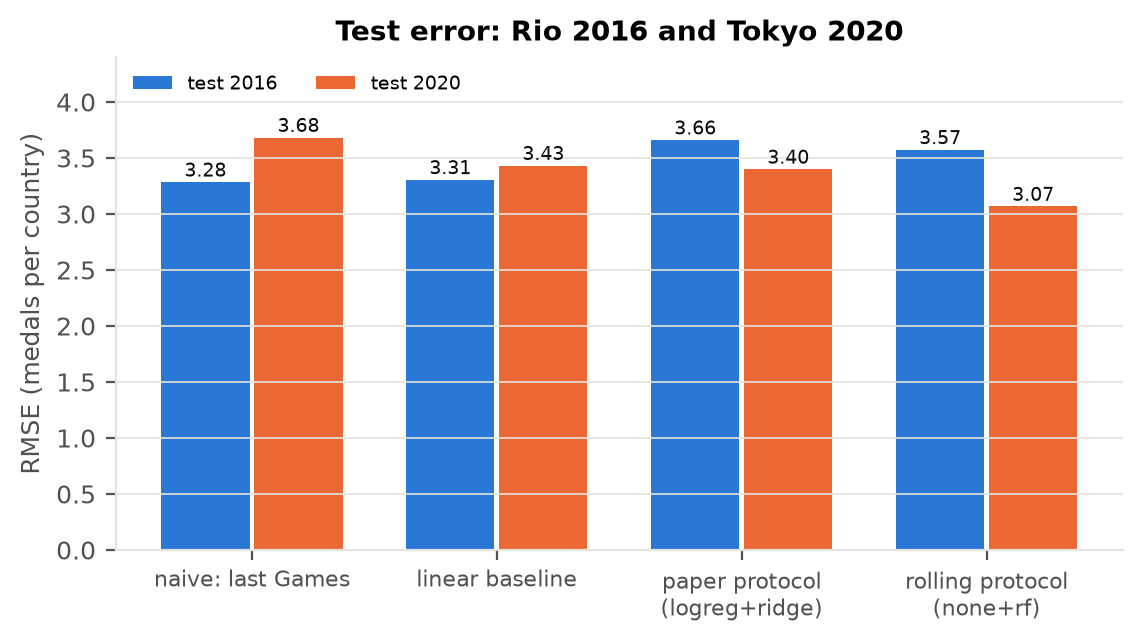
\includegraphics[width=\columnwidth]{../figures/fig_test_comparison.png}
\captionof{figure}{Test RMSE of the naive guess, the linear baseline and both selected models.}
\end{center}

\section*{6\quad Conclusions}
\begin{itemize}
\item On the real Tokyo 2020 results, economic indicators plus team size and past medals predict medal counts
  with an RMSE of about 3 medals per country, better than a linear baseline or ``same as last Games''.
\item The two-stage idea is not a general win. On rolling validation it helps Poisson (RMSE 12.90$\to$7.39) and
  SVR (3.52$\to$3.29), but for linear, ridge, lasso and random forest the single-stage model is as good or better.
  The single-stage forest was best overall, because it already predicts $\approx$0 for small countries.
\item Selecting on a single year is fragile. 2012 favoured ridge, while three validation years favoured random forests,
  which also did better on Tokyo.
\item The paper's headline 2016 number is most likely an evaluation on training data. Its protocol, applied to
  truly held-out data, does not beat the baseline. Medal counts are very persistent, and on 2016 no model beat
  ``same as last Games''.
\item Future work: impute missing indicators instead of dropping countries, use athlete-level form (recent world
  championships), and use a count-aware loss such as a zero-inflated or Tweedie model.
\end{itemize}
\end{multicols}
\end{document}
